\documentclass[]{book}
\usepackage{amsmath,amssymb}
\usepackage{amsthm}
\usepackage{xpatch}
\xpatchcmd\swappedhead{~}{.~}{}{}

\usepackage[T1]{fontenc}
\usepackage[utf8]{inputenc}

\usepackage{parskip}
\usepackage{lmodern}
\usepackage{enumerate}


\usepackage{xcolor}

\usepackage{hyperref}

\usepackage[ marginparwidth=3cm, marginparsep=0cm]{geometry}
\usepackage{graphicx}
\usepackage[spanish]{babel}


% Scale images if necessary, so that they will not overflow the page
% margins by default, and it is still possible to overwrite the defaults
% using explicit options in \includegraphics[width, height, ...]{}
\setkeys{Gin}{width=\maxwidth,height=\maxheight,keepaspectratio}
% Set default figure placement to htbp
\makeatletter
\def\fps@figure{htbp}
\makeatother


\providecommand{\tightlist}{%
  \setlength{\itemsep}{0pt}\setlength{\parskip}{0pt}}

  
%remove section numbers
%\setcounter{secnumdepth}{0}

\title{Introducción a la probabilidad}
\author{Hugo J. Bello}
\date{}


\renewcommand{\familydefault}{\sfdefault}
\setcounter{chapter}{2}


\theoremstyle{plain}
\swapnumbers % Switch number/label style
\newtheorem{theorem}{Teorema}[section]
\newtheorem{corollary}[theorem]{Corollary}
\newtheorem{lemma}[theorem]{Lemma}
\newtheorem{claim}{Claim}[theorem]
\newtheorem{axiom}[theorem]{Axiom}
\newtheorem{conjecture}[theorem]{Conjecture}
\newtheorem{fact}[theorem]{Fact}
\newtheorem{hypothesis}[theorem]{Hypothesis}
\newtheorem{assumption}[theorem]{Assumption}
\newtheorem{proposition}[theorem]{Proposition}
\newtheorem{properties}[theorem]{Propiedades}
\newtheorem{criterion}[theorem]{Criterion}

\theoremstyle{definition}
\newtheorem{definition}[theorem]{Definición}
\newtheorem{note}[theorem]{Nota}
\newtheorem{definitions}[theorem]{Definiciones}
\newtheorem{example}[theorem]{Ejemplo}
\newtheorem{remark}[theorem]{Remark}
\newtheorem{problem}[theorem]{Problem}
\newtheorem{principle}[theorem]{Principle}
\newtheorem{property}[theorem]{Propiedad}

\begin{document}
\chapter{Introducción a la probabilidad}

\section{Introducción y terminología}

\begin{definition}
La \textbf{probabilidad} puede ser entendida como una medida de la certidumbre de que ocurra un evento. 
Su valor es un número entre 0 y 1, 
donde un evento imposible corresponde a cero y uno seguro corresponde a uno.
\end{definition}

Una forma empírica de estimar la probabilidad consiste en obtener la 
frecuencia con la que sucede un determinado acontecimiento mediante la 
repetición de experimentos aleatorios, bajo condiciones suficientemente estables. 
En algunos experimentos de los que se conocen todos los resultados posibles, 
la probabilidad de estos sucesos pueden ser calculadas de manera teórica, 
especialmente cuando todos son igualmente probables.

La teoría de la probabilidad es la rama de la matemática que estudia los experimentos 
o fenómenos aleatorios. Se usa extensamente en áreas como la estadística, 
la física, las ciencias sociales, la Investigación médica, las finanzas, 
la economía y la filosofía para conocer la viabilidad de sucesos 
y la mecánica subyacente de sistemas complejos. 

\subsection*{Experimentos aleatorios}

\begin{definition}
Un \textbf{experimento aleatorio} es la reproducción controlada de un fenómeno, 
existiendo incertidumbre sobre el resultado que se obtendrá.
Un experimento aleatorio bajo el mismo conjunto aparente de condiciones iniciales, 
puede presentar resultados diferentes, es decir, no se puede predecir o reproducir 
el resultado exacto de cada experiencia particular. (Ej.: Lanzamiento de un dado,
lanzamiento de una moneda, lanzamiento de una carta de una baraja).

Este tipo de fenómeno es opuesto al suceso determinista, 
en el que conocer todos los factores de un experimento permite 
predecir exactamente el resultado del mismo. Por ejemplo, conociendo 
la altura desde la que se arroja un móvil es posible saber exactamente
el tiempo que tardará en llegar al suelo en condiciones de vacío. 
 Es al azar ya que es aleatorio. 
\end{definition}

\begin{example}
\begin{enumerate}
    \item Lanzar un dado de seis caras y anotar el resultado
    \item Preguntar su edad a cualquier persona que me encuentre y anotarla
    \item Lanzar una moneda y anotar si sale cara o cruz
    \item Lanzar 5 veces una moneda y anotar el número de caras
\end{enumerate}
\end{example}


\subsection*{Sucesos y el espacio muestral}

\begin{definition}
   Dado un experimento aleatorio, el \textbf{espacio muestral}  es 
   conjunto de todos los posibles resultados de un experimento aleatorio. Este conjunto se denota 
   por $\Omega$.
\end{definition}
Veamos varios ejemplos de espacios muestrales en distintos experimentos aleatorios
\begin{example}
  Veamos distintos ejemplos de experimentos aleatorios y espacios muestrales
        \begin{enumerate}
            \item Al Lanzar un dado de seis caras, tenemos el espacio muestral 
            \[\Omega = \{1, 2, 3, 4, 5, 6\}\]
            \item En el experimento preguntar su edad a cualquier persona que me encuentre y anotarla tenemos
            \[\Omega = \{0,1, 2, 3,\cdots, 130\}\]
            (suponiendo que la edad máxima de una persona sea 130)
            \item En el experimento lanzar una moneda y anotar si sale cara o cruz
            \[\Omega = \{C, X\}\]
            \item Lanzar 5 veces una moneda y anotar el número de caras
            \[\Omega = \{0, 1, 2, 3, 4, 5\}\]
        \end{enumerate}
\end{example}


\begin{definition}[Sucesos]
  Dado un experimento aleatorio, un \textbf{suceso}  cualquier conjunto de de resultados posibles del experimento.

Existen distintos tipos de sucesos

\begin{itemize}
  \item \textbf{Suceso seguro.} Es aquel que ocurre siempre. Por ejemplo, al tirar  una moneda, el suceso 
  \[A=\text{\emph{que salga cara o cruz}} = \{C, X\}\]
  El suceso formado por todo el espacio muestral es siempre un suceso seguro.
  
  \item \textbf{Suceso imposible.} Es aquel no ocurre nunca. Por ejemplo,  el suceso \emph{vacío},
  que en el experimento de tirar una moneda o un dado. Este suceso se representa por el conjunto vacío $\emptyset$.
  El suceso formado por todo el espacio muestral es siempre un suceso seguro.

  \item \textbf{Suceso simple.} Es aquel que no puede descomponerse. Por ejemplo en el experimento de tirar un dado, el suceso
  \[A=\text{\emph{que salga uno}} = \{1\}\]
  es simple.
  \item \textbf{Suceso compuesto.}  Es aquel que puede descomponerse en sucesos simples. Por ejemplo en el experimento de tirar un dado, el suceso
  \[A=\text{\emph{que salga uno o dos}} = \{1, 2\}\]
  es compuesto ya que podemos escribirlo como una unión de dos sucesos simples
  \[A= \{1, 2\} = \{1\} \cup \{2\}\]
  \item \textbf{Sucesos excluyentes.}  Dos sucesos $A$ y $B$ son excluyentes si se corresponden a resultados del experimento aleatorio que no pueden 
  darse nunca juntos, esto es $A\cap B = \emptyset$. Por ejemplo al tirar una moneda 
  \[A=\text{\emph{que salga cara}} = \{C\}\]
  \[B=\text{\emph{que salga cruz}} = \{X\}\]
  \[A\cap B=\text{\emph{que salga cara y cruz}} = \{C\} \cap \{X\} = \emptyset\]
  Por lo tanto el los sucesos $A$ y $B$ son excluyentes.
  \item  \textbf{Suceso complementario.} Dado un suceso $A$, su complementario es el suceso formado 
  por el conjunto complementario $A^c$
\end{itemize}

\end{definition}


\begin{note}[Recordatorio conjuntos]
  Recordemos que 
  \begin{itemize}
    \item La \textbf{unión} de dos conjuntos $A$ y $B$ se denota por $A\cup B$ y es el conjunto formado por los 
    elementos que están en $A$ \textbf{o} en $B$.
    \item La \textbf{intersección} de dos conjuntos $A$ y $B$ se denota por $A\cap B$ y es el conjunto formado por los 
    elementos que están en $A$ \textbf{y} en $B$.
    \item El conjunto vacío $\emptyset$ es aquel que no tiene ningún elemento.
    \item Dado un conjunto $A$, su \textbf{complementario} (dentro de un conjunto universo $\Omega$) lo conforman los elementos 
    \emph{que no están en $A$}.
    \item Dos conjuntos $A$ y $B$ son \textbf{disjuntos} si no tienen elementos en común, esto es 
    \[
    A \cap B = \emptyset  
    \]

    \item Un conjunto $A$ es un \textbf{subconjunto} de $B$ si todo elemento de $A$ es un elemento de $B$. En este caso escribiremos
    $A\subset B$.
    
    \item Dados dos conjuntos $A$ y $B$ la \textbf{resta} de conjuntos $A-B$ se define como los elementos de $A$ que no están en $B$.
    \end{itemize}

    \begin{figure}[htbp]
      \begin{minipage}{0.5\linewidth}
      \centering
      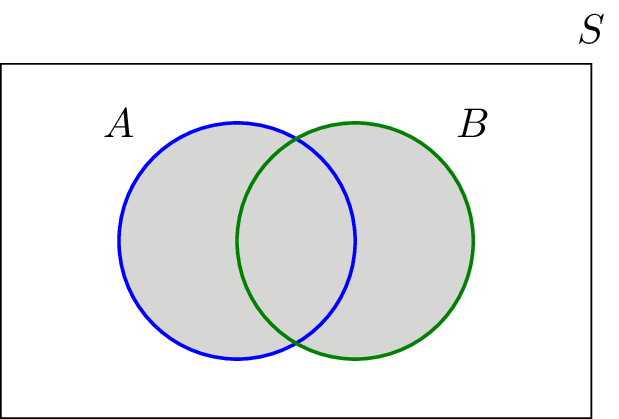
\includegraphics[width=1.5in,height=\textheight]{img/union_b.png}
      \caption{Unión de conjuntos}
      \end{minipage}%
      \begin{minipage}{0.5\linewidth}
      \centering
      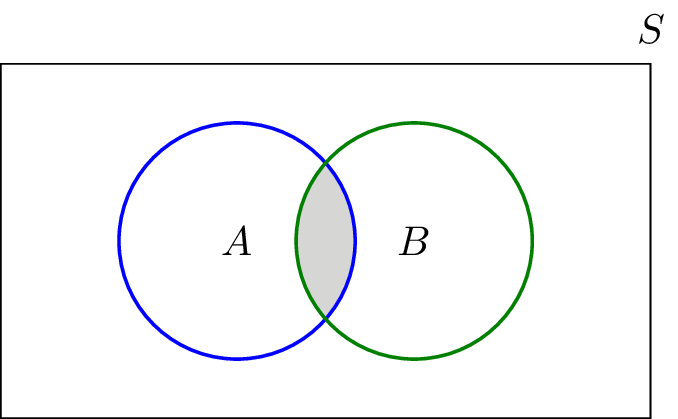
\includegraphics[width=1.5in,height=\textheight]{img/intersection_b.png}
      \caption{Intersección de conjuntos}
      \end{minipage}

      \begin{minipage}{0.5\linewidth}
      \centering
      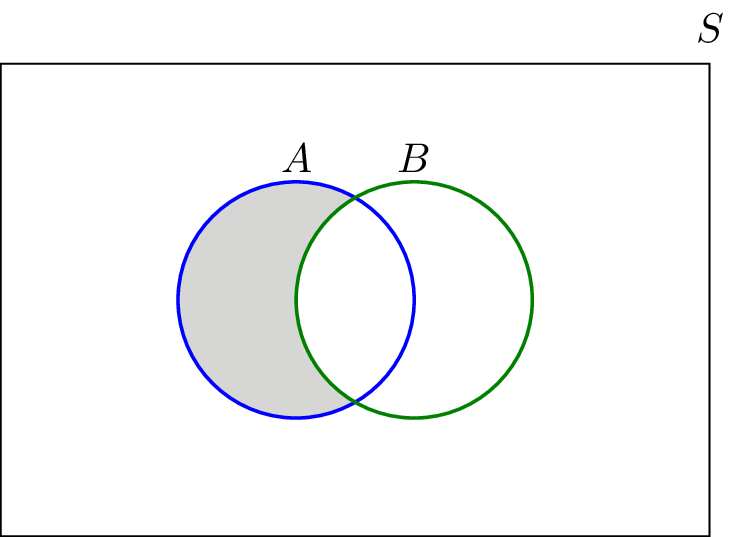
\includegraphics[width=1.5in,height=\textheight]{img/difference_b.png}
      \caption{Resta de conjuntos}
      \end{minipage}%
      \begin{minipage}{0.5\linewidth}
      \centering
      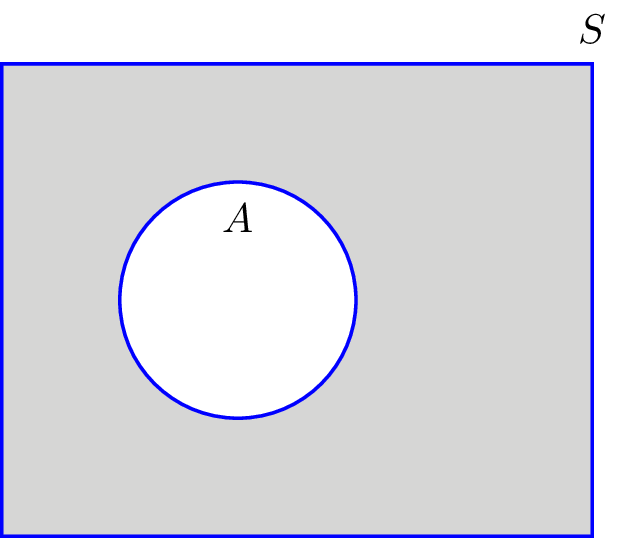
\includegraphics[width=1in,height=\textheight]{img/complement_b.png}
      \caption{Complementario de conjunto}
      \end{minipage}
    \end{figure} 
\end{note}


\newpage
\section{Definición de probabilidad y sus propiedades}

Definir de manera formal la probabilidad require conocimientos que se salen de lo que se intenta transmitir aquí. Daremos una aproximación
al concepto de probabilidad a través de sus propiedades.

A un nivel intuitivo, dado un experimento aleatorio y un suceso $A\in \Omega$, la \textbf{probabilidad} de $A$,
es un número entre $0$ y $1$ que denotaremos por $P(A)$ y que expresa 
\begin{itemize}
  \item la frecuencia relativa con la que se presenta el suceso (al repetir el experimento si esto fuera posible)
  \item la proporción o cociente entre el número de resultados que forma el suceso y el número de sucesos posibles del experimento.
  \item el grado de creencia o certeza que tenemos de la ocurrencia del suceso.
\end{itemize}

La manera en que se define la propiedad es a través de sus axiomas, que son tres. 

\begin{definition}[Axiomas de la probabilidad]\label{def_axiom}
Dado un espacio muestral $\Omega$, la probabilidad asigna a cada $A\in \Omega$ un número
$P(A)$ que cumple
\begin{enumerate}
  \item[i.] $P(A)$ está entre $0$ y $1$
  \item[ii.] $P(\Omega) = 1$
  \item[iii.] Si $A$ y $B$ son sucesos excluyentes (esto es, $A\cap B = \emptyset$) entonces $P(A\cup B) = P(A) + P(B)$.
\end{enumerate}
\end{definition}

\begin{property}
  De los axiomas de la probabilidad se deducen las siguientes propiedades
\begin{enumerate}[(1)]
  \item Si $A_1, A_2, \ldots A_n$ son sucesos excluyentes dos a dos \footnote{esto es, dados dos cuales quiera de ellos $A_i, A_j$, no tienen elementos en común, es decir $A_i\cap A_j = \emptyset$}
  Entonces $$P(A_1 \cup A_2, \ldots, A_n)=P(A_1) + P(A_2) + \ldots P(A_n)$$
  Esta propiedad símplemente generaliza \ref{def_axiom}.iii y se deduce de esta.
  \item Para cualquier suceso $A\in \omega$, se cumple
  \begin{equation}\label{eq_compl}
    P(A^c) = 1-P(A)
  \end{equation}
  Para convencernos de esto basta observar de que $A$ y $A^c$ son siempre sucesos excluyentes, 
  por otra parte puesto que $\Omega = A \cup A^c$, por la propiedades \ref{def_axiom}.ii y \ref{def_axiom}.iii se deduce esta propiedad \ref{eq_compl}. 
  \item Se cumple
  \[P(\emptyset) = 0 \]
  esto se deduce de \ref{def_axiom}.ii, dado que $\emptyset$ y $\Omega$ son complementarios.
  \item Para cualesquiera sucesos $A,B\in \Omega$
  \[P(A-B)= P(A) - P(A\cap B)\]
  Esto se deduce de que $A$ puede ponerse como unión de dos conjuntos disjuntos de la siguiente manera $A = A \cup (A-B)$
  \item Para cualesquiera sucesos $A,B\in \Omega$
  \[P(A\cup B) = P(A) + P(B) - P(A\cap B)\]
  \footnote{para deducir esto podemos observar que $A\cup B $ se puede poner como unión de tres sucesos excluyentes (conjuntos disjuntos) de la siguiente manera 
   $A\cup B = (A-B) \cup (A\cap B) \cup (B-A)$ de modo que la probabilidad de $A\cup B$ será la suma de estas tres probabilidades, es decir 
   \[P(A\cup B) = P(A-B) - P(A\cap B) + P(A\cap B) + P(B) - P(A\cap B) = P(A) + P(B) - P(A\cap B) \]}
\end{enumerate}
\end{property}


\section{Ley de Laplace}

\begin{theorem}[Ley de Laplace]\label{th_laplace}
  Si realizamos un experimento aleatorio en el que hay $n$ sucesos 
  simples, todos igualmente probables (equiprobables), 
  entonces si $A$ es un suceso, 
  la probabilidad de que ocurra el suceso $A$ es:
  \begin{equation}\label{equ_array}
    P(A) = \frac{\text{número de casos favorables para que ocurra A}}{\text{número de casos posibles para que ocurra A}}
  \end{equation}
\end{theorem}

\begin{example}
  Hallar la probabilidad de que al lanzar dos monedas al aire salgan dos caras
  Llamemos $A$ al suceso \emph{salgan dos caras}
  
  Los casos favorables para $A$, serán solo: cc.

  Los casos posibles para $A$ serán : cc, cx, xc, xx.
  
  Aplicando la Ley de Laplace la probabilidad
  \[     P(A) = \frac{\text{número de casos favorables para que ocurra A}}{\text{número de casos posibles para que ocurra A}} = \frac{1}{4}\]
\end{example}


\begin{example}
  Hallar la probabilidad de que al lanzar dos monedas al aire salgan dos caras
  Llamemos $A$ al suceso \emph{salgan dos caras}
  
  Los casos favorables para $A$, serán solo: cc.

  Los casos posibles para $A$ serán : cc, cx, xc, xx.
  
  Aplicando la Ley de Laplace la probabilidad \ref{th_laplace}
  \[     P(A) = \frac{\text{número de casos favorables para que ocurra A}}{\text{número de casos posibles para que ocurra A}} = \frac{1}{4}\]
\end{example}

\begin{example}
  Calcular la probabilidad de que al echar un dado al aire, salga:
\begin{enumerate}[(1)]
  \item Un número par
  \item Un múltiplo de tres
  \item Un número mayor que 4
\end{enumerate}
Para $(1)$
llamemos \[A=\text{que salga par}\]

Casos favorables para $A$: 2, 4, 6.

Casos posibles para $A$: 1, 2, 3, 4, 5, 6.

Aplicando \ref{th_laplace}

$$\displaystyle \text{P(A)}=\frac{3}{6}=\frac{1}{2}$$

Para $(2)$
llamemos \[B=\text{que salga múltiplo de 3}\]

Casos favorables para $B$: 3, 6.

Casos posibles para $B$: 1, 2, 3, 4, 5, 6.

Aplicando \ref{th_laplace}

$$\displaystyle \text{P(B)}=\frac{2}{6}=\frac{1}{3}$$

Para $(3)$ llamemos 
\[C = \text{que salga mayor que 4}\]

Casos favorables para C: 5, 6.

Casos posibles para C: 1, 2, 3, 4, 5, 6

Aplicando \ref{th_laplace}

$$\displaystyle \text{P(C)}=\frac{2}{6}=\frac{1}{3}$$

\end{example}




\begin{note}[Repaso combinatoria, conteo sencillo]

A menudo necesitaremos contar el número de maneras posibles en que podemos
ordenar o seleccionar subconjuntos de un conjunto. Esto require hablar de \textbf{combinatoria}.
La combinatoria tiene mucha terminología, en muchas ocasiones podemos 
realizar conteos de manera intuitiva teniendo en cuenta el truco que vamos a explicar a continuación. 

Si queremos contar las maneras de $k$ elementos de un conjunto de $n$ teniendo en cuenta el orden podemos 
comprenderlo bien através de los siguiente ejemplos

\begin{itemize}
  \item Supongamos que queremos contar las \textbf{maneras posibles de formar números de 2 dígitos permitiendo repeticiones} podemos observar como 
tenemos dos \emph{espacios} o \emph{huecos}, uno por cáda dígito, y podemos elegir 
de entre 10 elementos en el primero y 10 en el segundo

\begin{figure}[htbp]
  \centering
  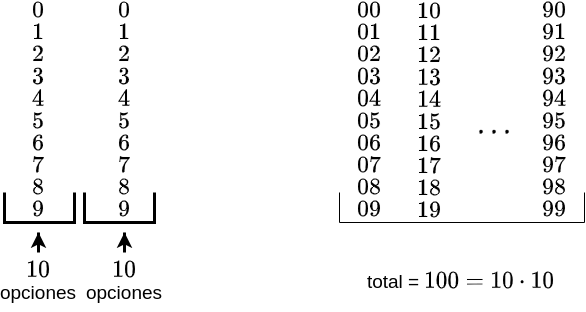
\includegraphics[width=3.5in,height=\textheight]{img/conteo_basico_1.png}
  \caption{truco para contar las maneras de formar números de dos dígitos permitiendo repeticiones}
  \end{figure}%
  
Con lo cual al final esto nos resulta en 100 posibilidades. Esto se puede entender escribiéndolas o pensando que son 10 por cada \emph{hueco posible}

\item Si queremos contar las \textbf{maneras posibles de formar números de 3 dígitos permitiendo repeticiones} la historia es similar

\begin{figure}[htbp]
  \centering
  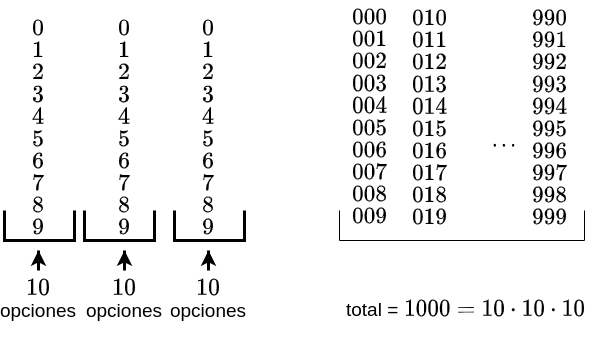
\includegraphics[width=3.5in,height=\textheight]{img/conteo_basico_2.png}
  \caption{truco para contar las maneras de formar números de 3 dígitos permitiendo repeticiones}
  \end{figure}%
  
Vemos que es la misma idea, basta multiplicar el número de opciones que tenemos en cada \emph{hueco}. En este caso 10 en el primero, 10 en el segundo y otras 10 en el tercero.

\item Otro caso es pensar en hacer esto pero sin repetir ningún dígito, es decir contar las \textbf{maneras posibles de formar números de 3 dígitos sin repeticiones}

\begin{figure}[htbp]
  \centering
  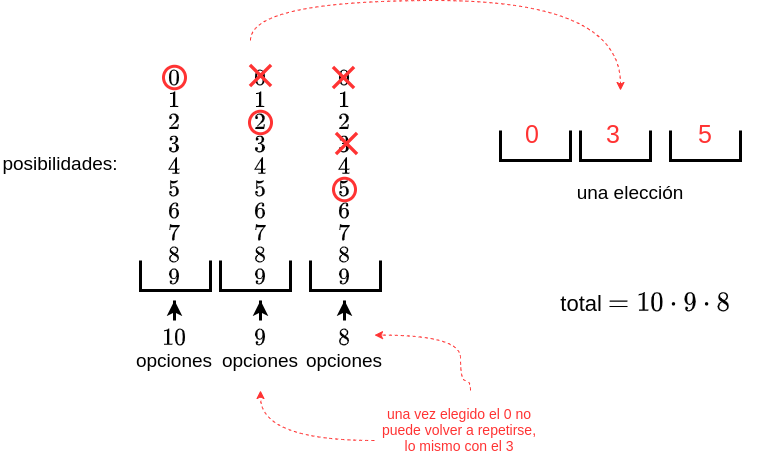
\includegraphics[width=3.5in,height=\textheight]{img/conteo_basico_3.png}
  \caption{truco para contar las maneras de formar números de 3 dígitos sin repeticiones}
  \end{figure}%

Como vemos, con cada elección las opciones merman, ya que no podemos repetir. De modo que en el primer hueco tenemos $10$ opciones, en el segundo $9$ y en el tercero $8$. El resultado 
será $10 \cdot 9 \cdot 8$. 

\item En general hemos aprendido el siguente \textbf{truco}. \emph{Si tenemos un conjunto de $n$ elementos y tenemos que elegir $k$ importando el orden},
 lo que tendremos que hacer para averiguar el total de maneras de hacer esto es:

\begin{figure}[htbp]
  \centering
  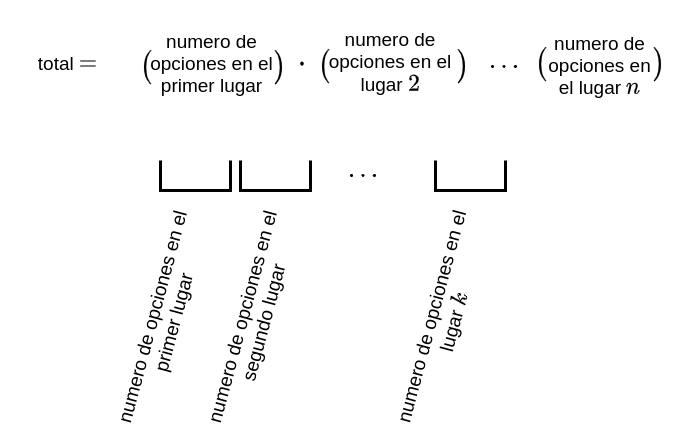
\includegraphics[width=3.5in,height=\textheight]{img/conteo_basico_4.png}
  \caption{truco para contar las maneras de formar números de 3 dígitos sin repeticiones}
  \end{figure}%

\end{itemize}

\end{note}


\begin{note}[Repaso combinatoria, combinaciones]

En los ejemplos anteriores nos centramos en el conteo de maneras de formar subconjuntos de tal manera que importaba el orden, pero ¿Cómo lo podemos hacer si el orden no importa?

Por ejemplo, Si quiero repartir 2 premios iguales a 2 personas distintas de una clase de 30 alumnas de cuántas maneras puedo hacerlo. 
Aquí vemos como  da lo mismo el orden en que reparta los premios ya que son iguales (no hay un primero y segundo).

En este caso estamos ante las combinaciones de 10 elementos tomados de 2 en 2.

Se llama \textbf{combinaciones} de $n$ elementos tomados de  $k$ en $k$
a todas las agrupaciones posibles que pueden hacerse con los 
$k$ elementos de forma que:
\begin{itemize}
  \item No importa el orden
  \item No se repiten los elementos
\end{itemize}

Y el total de formas de hacer esto es justamente
\[{n \choose k} = \frac{n!}{(n-k)! k!}\]

Donde el símbolo $!$ es el \emph{factorial} y se calcula de la siguiente manera:

\[n! = n \cdot (n-1) \cdot (n-2) \cdot \ldots \cdot 1\]

En el ejemplo anterior tendríamos 

\[{10 \choose 2} = \frac{10!}{(10-2)! 2!} = \frac{10!}{(8)! 2!} = 5\cdot 9 = 45\]


\begin{example}
  Una empresa quiere repartir 3 premios entre los 200 usuarios de su web. Los premios son iguales y cada usuario puede recibir a lo sumo 1 premio.
  Si una persona tiene 1 usuario registrado en la web, ¿Qué posibilidades tiene de ganar un premio? 

  Para resolver esto llamemos
  $$A=\text{ganar un premio teniendo 1 usuario}$$

\begin{align*}
  \text{casos posibles}&= \text{maneras de seleccionar 3 ganadores entre 200}\\
  &={200 \choose 3} = \frac{200 \cdot 199 \cdot 198 \cdot 197 \cdot \ldots 1 }{(197 \cdot \ldots 1)\cdot 3\cdot 2} = \frac{200 \cdot 199 \cdot 198}{6} = 1313400
\end{align*}

Esto se debe a que al seleccionar esos 3 ganadores los conformamos sin importar el orden (son todos los premios iguales) y sin repetición (no damos dos premios al mismo usuario)
  
Veamos los casos favorables: 

\begin{align*}
  \text{casos favorables para A}&= \text{maneras de que el usuario esté entre los 3 ganadores}\\
  &= \text{maneras de elegir a los otros dos ganadores a parte del nuestro}\\
  &={200 \choose 2} = \frac{200!}{(200-2)! \cdot 2!} = \frac{200 \cdot 199 \cdot 198 \cdot \ldots 1 }{(198 \cdot \ldots 1)\cdot 2} = \frac{200 \cdot 199}{2}= 19900
\end{align*}

El hecho de que se reduzca a calcular maneras de elegir a los otros dos ganadores a parte del nuestro, es porque al asumir que $A$ ha ocurrido ya sabemos que nuestro usuario
está entre los 3, de modo que basta con calcular las maneras en que podemos elegir a los otros 2.

Con lo cual, usando la regla de Laplace

\[P(A) = \frac{\text{número de casos favorables para que ocurra A}}{\text{número de casos posibles para que ocurra A}} = \frac{19900}{1313400}\cong 0.015\]

\end{example}



\end{note}


\end{document}